\section{Recurrent translation models} \label{RNN}

In this section, we discuss a category of neural models that are effective in modeling languages. 
Earlier developments of neural models addressing language modeling tasks incorporated the temporal structure of the language in the structure of the network \citep{Jacquemin1994ATC,Schmidhuber:HabilitationThesis}.  
A recurrent neural network (RNN) is an example of these sequential models \citep{10.5555/65669.104451}.
RNNs are powerful models that achieve state-of-the-art results in a variety of tasks such as question answering \citep{garg2019tanda}, reading comprehension \citep{Zhang2020RetrospectiveRF}, image semantic segmentation \citep{yuan2019objectcontextual}, and speech recognition \citep{8049322}. 

RNN models are capable of modeling sequences of text with various length, while selectively passing on information between different time steps in the sequence. 
A long short-term memory (LSTM) network \citep{hochreiter1997long} is an RNN structure that uses special LSTM units in addition to standard ones. 
These special units include a memory cell that can maintain information for long sequences.
LSTM models address the \textit{vanishing gradient problem} in the earlier RNN architecture where the weights and biases of the hidden layers are not updated effectively because the gradient decreases exponentially \citep{10.1142/S0218488598000094}. 

\begin{figure}[htb!]
\centering
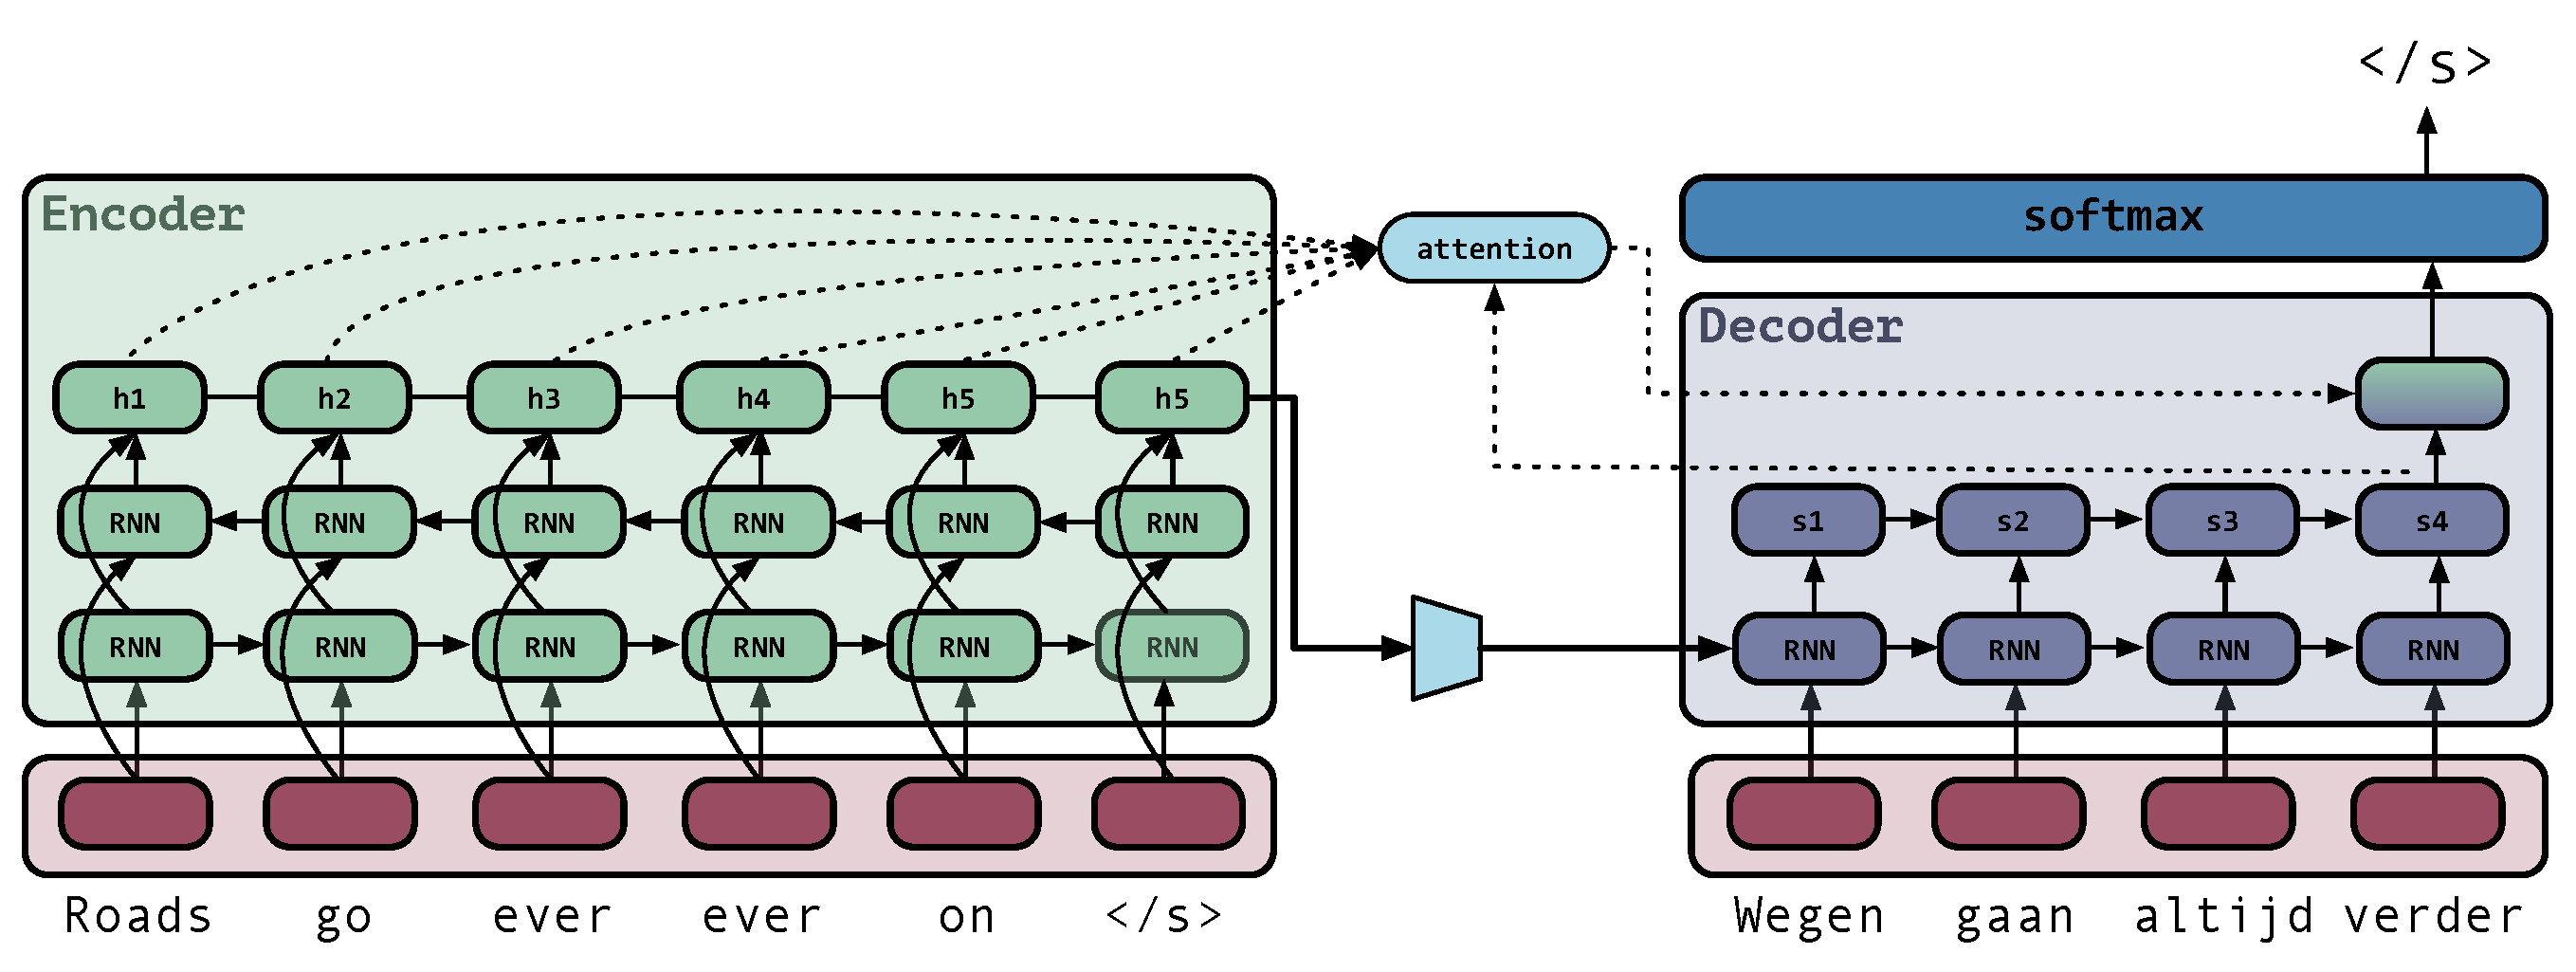
\includegraphics[width=0.95\linewidth]{02-background/figs/rnnarc.pdf}
\caption{An illustration of an RNN encoder-decoder with attention.}
\label{bgRNNfig}
\end{figure}

\citet{sutskever2014sequence} and \citet{cho2014properties} were among the firsts to employ RNNs to build an end-to-end machine translation model.
\citet{DBLP:journals/corr/BahdanauCB14} and \citet{luong:2015:EMNLP} introduced an \textit{attention mechanism} that achieved performance on par with traditional statistical models. 
In the following sections, we describe the RNN architecture with attention used in the NMT experiments in this thesis. 


\subsection{Model architecture}

Neural machine translation models fall under a sequence-to-sequence framework where an encoder builds up a representation of the source sentence and a decoder 
generates the target translation. 
Both the encoder and the decoder can be recurrent neural models.
Figure~\ref{bgRNNfig} illustrates this architecture which we will discuss in detail in this section. 
%
In order to train an NMT system, two sequences of tokens, $X =  \big[ x_1, \ldots, x_n \big] $ and $Y =  \big[ y_1, \ldots, y_m \big] $, are given in the source and target language, respectively.
As discussed in Section~\ref{bgemb}, the input tokens are mapped to an embedding space.
As a result, the source sequence is the input to the encoder as vectors: $\big[ \vt{x}_1, \ldots, \vt{x}_n \big]$.

The encoder then encodes the input sequence into hidden states, where at time step $t$ the hidden state is a function of the current input vector and the previous hidden state:
\begin{align}
\vt{h}_t = f(\vt{x}_t, \vt{h}_{t-1})
\end{align}

Function $f$ adds non-linearities to the transformation of the input sequence to the output of the encoder.
With a bidirectional architecture, two RNNs are run on the input sequence: one in forward and one in backward direction. The hidden state at time $t$ is created by concatenating the forward and backward hidden states
at each point in time, the input has access to the information on both sides. 
Note that the forward and backward hidden states are concatenated to create the top hidden states of the encoder, $\vt{h}_t$ as follows:
\begin{align}
\vt{h}_t = \big[ \overrightarrow{\vt{h}_t}^\intercal; \overleftarrow{\vt{h}_t}^\intercal \big]^\intercal,      t = 1, \ldots, n
\end{align}

%%%%%%%%%%%%%%%%%%

The decoder then generates the target translation one word at a time starting with the last hidden state of the encoder and the representation for the start-of-sentence symbol \mbox{\texttt{\textless s\textgreater}}.
Each decoder hidden state $\vt{s}_t$ is computed as:
\begin{align}
\vt{s}_t = g(\vt{s}_{t-1}, \vt{y}_{t-1}, \vt{c}_t)
\end{align}

\noindent where $g$ is a transformation function that outputs a vocabulary-sized vector and $\vt{y}_{t-1}$ is the representation of the previously predicted token.
$\vt{c}_i$ is the context vector for output at position $i$ and is defined as:
\begin{align}
\vt{c}_i = \sum_{j=1}^{n} \alpha_{ij} \vt{h}_j
\end{align}

This context vector is recomputed at each time step.
$\alpha_{ij}$ is the attention weight and it is computed for all source words at each time step $i$.
We will discuss different approaches to computing attention weights in Section~\ref{BGlstmATT}.

Next, the decoder predicts each target token $y_t$ by computing the conditional probability:
\begin{align}
p(y_t \mid y_{<t}, X) = \softmax \,(\vt{s}_t)
\end{align}

This conditional probability is computed over the vocabulary of the target language which is fixed during training and testing. 
For token $y_t$, the conditional probability $p(y_t \mid y_{<t}, X)$ during training quantifies the difficulty of predicting that token in the context $y_{<t}$.
The prediction loss of token $y_t$ is the negative log-likelihood of this probability.
During training on a parallel corpus $\mathbb{D}$, the cross-entropy objective function is defined as:
\begin{align}
\mathcal{L} = \sum_{(X,Y) \in \mathbb{D}} \sum_{i=1}^{m} - \log p(y_i \mid y_{<i}, X)
\end{align}

The objective of this function is to improve the model's estimation of predicting target words given the source sentence and the target context. 
The model is trained end-to-end by minimizing the negative log-likelihood of the target words using stochastic gradient descent.

NMT systems often benefit from multiple layers of stacked RNNs during training \citep{wu2016google}. 
By increasing the number of parameters, the learning capability of the model also increases \citep{britz-etal-2017-massive}.
\citet{belinkov-etal-2017-neural} show that different layers in the encoder capture different linguistic features, namely that higher layers capture semantics while lower layers tend to capture syntax.
Encoding the input sequence in both directions also provides advantages \citep{luong:2015:EMNLP,DBLP:journals/corr/BahdanauCB14}. The backward layer in a recurrent model learns more about the semantics of words, whereas the forward layer encodes more of the local context \citep{ghader-monz-2019-intrinsic}.

\subsection{Inference} \label{bgrnninference}

During inference, a trained model is given a source sentence and it generates the target translation word by word using a left-to-right beam search technique \citep{jelinek98}
This procedure was already adopted by pre-neural translation methods such as phrase-based translation models \citep{koehn-etal-2003-statistical}. 
Generation of target words stops when a special end-of-sentence symbol \mbox{\texttt{\textless /s\textgreater}} is generated. 
At each step, the model computes a probability distribution over all words in the target language and chooses the most likely word:
\begin{align}
\hat{Y} = \underset{Y}\argmax \; p({Y} \mid {X})
\end{align}

\citet{sutskever2014sequence} showed that increasing the beam size beyond 2 does not improve the predictions significantly and even with a beam size of 1, the model performs well. 
With a large enough beam size, the best translation performance can be reached with the drawback of efficiency \citep{freitag-al-onaizan-2017-beam}.
It is common practice to set beam size to around 5 to 10 \citep{wu2016google,edunov-etal-2018-understanding}.
Beam search decoding, even though effective, still suffers from \textit{exposure bias}.
Exposure bias results from the mismatch between how the models are trained and how they are used at inference \citep{wiseman-rush-2016-sequence,DBLP:journals/corr/RanzatoCAZ15}.
During training, the model is guided by the ground-truth target translation. 
However, at inference, target translations are not available and the model has to rely on its own predictions which can be wrong.
\citet{collobert2019a} proposed a fully differentiable beam search decoder that can be used during training and eliminates this bias.


\subsection{Attention mechanism} \label{BGlstmATT}

One of the shortcomings of the discussed models is that the translation quality decreases considerably as sentences become longer \citep{koehn2017six}.
One reason is that the source sentence is encoded into one \textit{fixed length} vector and this vector is expected to be a complete and static representation of the source sentence.
To address this problem, several works focus on learning a context vector with connections to the source sentence \citep{Graves2014NeuralTM,DBLP:journals/corr/BahdanauCB14,luong:2015:EMNLP}. 
This context vector regulates the alignment between the source and the target sentences and is a sum of the hidden states of the input, weighted by alignment scores.
At each time step $t$, the model computes a variable-length alignment weight vector based on the current target state and all source inputs. 
Table~\ref{backgroundattentions} summarizes different approaches for computing alignment scores.

\begin{table}
\centering
\small
\begin{tabularx}{0.93\linewidth}{lll}
 \toprule
\textbf{Name} & \textbf{Proposed by} & \textbf{Alignment score}  \\ \midrule
Additive & \citet{DBLP:journals/corr/BahdanauCB14} & $\text{score}(\vt{s}_i, \vt{h}_t) = \vt{v}^\intercal_a \tanh (\vt{W}_a[\vt{s}_i, \vt{h}_t])$ \\
 Location-base	 & \citet{luong:2015:EMNLP} & $\alpha_{n, t} = \softmax\,(\vt{W}_a\vt{s}_i) $ \\
General	 &  \citet{luong:2015:EMNLP} & $ \text{score}(\vt{s}_i, \vt{h}_t) = \vt{s}^\intercal_i  \vt{W}_a  \vt{h}_t $ \\
Dot-product	 &  \citet{luong:2015:EMNLP} & $\text{score}(\vt{s}_i, \vt{h}_t) = \vt{s}^\intercal_i \vt{h}_t  $ \\
 Scaled dot-product & \citet{vaswani2017attention} & $\text{score}(\vt{s}_i, \vt{h}_t) = \frac{\vt{s}^\intercal_i \vt{h}_t }{\sqrt{n}} $ \\
\bottomrule
\end{tabularx}
\caption{Different alignment scores in the literature used for creating the context vector. }
\label{backgroundattentions}
\end{table}

It is worth noting that while attention matches traditional word alignment at times, it often captures relations beyond that between the source and target sentence \citep{ghader-monz-2017-attention,koehn2017six}.

